\section{Introduction}
The binary search tree (BST) model is one of the most fundamental and thoroughly studied data access models in computer science. 
In this model, given a sequence $X \in [n]^m$ of keys, we are interested in $\OPT(X)$, the optimum cost of accessing $X$ by a binary search tree. When the tree does not change between accesses, $\OPT$ is well understood: both efficient exact algorithms (Knuth~\cite{knuth_optimum}) and a linear time approximation (Mehlhorn~\cite{mehlhorn1975nearly}) have long been known. By contrast, in the dynamic BST model (where restructuring of the tree is allowed between accesses) our understanding of $\OPT$ is very limited. No polynomial time exact or constant-approximation algorithms are known for computing $\OPT$ in the dynamic BST model.


Theoretical interest in the dynamic BST model is partly due to the fact that it holds the possibility of a meaningful ``instance optimality'', i.e.\ of a BST algorithm that is constant factor competitive (in the amortized sense) with any other BST algorithm, even with those that are allowed to see into the future. 
The existence of such a ``dynamically optimal'' algorithm has been postulated in 1985 by Sleator and Tarjan~\cite{ST85}; they conjectured their splay tree to have this property. 
Later, Lucas~\cite{Luc88} and independently Munro~\cite{Mun00} proposed a greedy offline algorithm as another candidate for dynamic optimality. 
In 2009 Demaine, Harmon, Iacono, Kane, and P\u{a}tra\c{s}cu (DHIKP)~\cite{DHIKP09} presented a geometric view of the BST model, in which the Lucas-Munro offline algorithm naturally turns into an online one (simply called {\sc Greedy}).  
Both splay and \greedy are considered plausible candidates for achieving optimality. However, despite decades of research, neither of the two algorithms are known to be $o(\log n)$-competitive (the best known approximation ratio for any BST is $O(\log \log n)$~\cite{tango}, but the algorithms achieving this bound are less natural). Thus, the dynamic optimality conjecture remains wide open.


Why is dynamic optimality difficult to prove (or disprove)? For a vast majority of access sequences, the optimal access cost by any dynamic BST (online or offline) is\footnote{This observation appears to be folklore. We include a proof in Appendix~\ref{sec:random-hard}.} $\Theta(m \log n)$ 
and any static balanced tree can achieve this bound.\footnote{As customary, we only consider successful accesses, we ignore inserts and deletes, and we assume that $m \geq n$. }
Hence, dynamic optimality is almost trivial on most sequences. However, when an input sequence has complexity $o(m \log n)$, a candidate BST must ``learn'' and ``exploit'' the specific structure of the sequence, in order to match the optimum. This observation motivates the popular research direction that aims at understanding ``easy'' sequences, i.e.\ those with $\opt = O(m d)$ when $d$ is a parameter that depends on the structure of the sequence; typically $d=o(\log n)$. 
Parameter $d$ can be seen as a measure of ``easiness'', and the objective is to prove that a candidate algorithm achieves the absolute bound of $O(m d)$; note that this does not immediately imply that the algorithm matches the optimum.

The splay tree is known to perform very well on many ``easy'' sequences: It achieves the access time of $O(m d)$ when $d$ is a parameter that roughly captures the average distances between consecutive accesses~\cite{finger1,finger2}, the average entropy, or the recentness of the previous accesses~\cite{ST85}; these properties are called {\em dynamic finger}, {\em static optimality} and {\em working set} bounds respectively (the latter two bounds are also satisfied by \greedy~\cite{Fox11}). %Furthermore, both splay and \greedy can access the keys in a monotone sequence in the optimal $O(n)$ time~\cite{tarjan_sequential, Fox11} ({\em sequential access}). 
The notorious difficulty of dynamic optimality is perhaps witnessed by the fact that many other highly restricted special cases have resisted attempts and remain unresolved. These special cases stand as a roadblock to proving (or disproving) the optimality of any algorithm: proving that $\mathcal{A}$ is optimal requires proving that it performs well on the easy inputs; refuting the optimality of $\mathcal{A}$ requires a special ``easy'' subclass %i.e.\ one with $\opt = o(m \log n)$, 
on which $\mathcal{A}$ is provably inefficient. In any case, a better understanding of easy sequences is needed, but currently lacking, as observed by several authors~\cite{DHIKP09,deque_Pet08}.%% (``there is currently no {\em theory} of access sequences whose inherent complexity is linear.'')
  
 
One famous example of such roadblocks is the {\em traversal conjecture}, proposed by Sleator and Tarjan in 1985.  
This conjecture states that starting with an arbitrary tree $T$ (called {\em initial tree}) and accessing its keys using the splay algorithm in the order given by the preorder sequence of another tree $T'$ takes linear time.
Since the optimum of such preorder sequences is linear, any dynamically optimal algorithm must match this bound.  
After three decades, only very special cases of this conjecture are known to hold, namely when $T'$ is a monotone path (the so-called \emph{sequential access}~\cite{tarjan_sequential})
or when $T'= T$~\cite{chaudhuri}.\footnote{This result implies an offline BST with $O(n)$ cost for accessing a preorder sequence, by first rotating $T$ to $T'$.}
Prior to this work, no online BST algorithm was known to be linear on such access sequences. 


\begin{table} 
\scriptsize\centering 
\begin{tabular}{|>{\raggedright}p{0.08\paperwidth}|>{\raggedright}p{0.15\paperwidth}|>{\centering}p{0.2\paperwidth}|>{\centering}p{0.16\paperwidth}|>{\centering}p{0.13\paperwidth}|}
\hline 
 & Structure  & splay bound & \greedy bound & Remark \tabularnewline
\hline 
\hline 
Static optimality & low entropy & $O(\sum_{i=1}^{n}f_{i}(1+\log\frac{m}{f_{i}}))$ \\~\cite{ST85}& same as splay ~\cite{Fox11, our_icalp} & \multirow{2}{0.1\paperwidth}{corollaries of Access~Lemma \cite{ST85}} \tabularnewline
\cline{1-4} 
Working set  & temporal locality & $O(m+n\log n+\sum_{t=1}^{m}\log(\tau_{t}+1))$\\ ~\cite{ST85}&  same as splay ~\cite{Fox11, our_icalp}& \tabularnewline
\hline 
Dynamic finger  & key-space locality & $O(m+\sum_{t=2}^{m}\log|x_{t}-x_{t-1}|)$\\~\cite{finger1,finger2} & ? & \tabularnewline
\hline
Deque  & $n$ updates at min/max elements & $O(n\alpha^{*}(n))$ ~\cite{deque_Pet08} & $O(n2^{\alpha(n)})$ ~\cite{our_wads}& $O(n)$ for multi-splay~\cite{multisplay} from empty tree \tabularnewline
\hline 
Sequential  & avoid $(2,1)$ & $O(n)$~\cite{tarjan_sequential, pettie_DS} & $O(n)$~\cite{Fox11, our_wads} & \tabularnewline
\hline 
Traversal  & avoid $(2,3,1)$ & ? & $n2^{\alpha(n)^{O(1)}}$ [* Cor~\ref{cor:trav1}] & $\opt = O(n)$ \tabularnewline
\hline 
\multirow{4}{0.07\paperwidth}{Pattern-avoiding (new)} & avoid $(2,3,1)$ with preprocessing & ? & $O(n)$ [* Cor~\ref{cor:trav2}] & $\opt = O(n)$ \tabularnewline
\cline{2-5} 
 & avoid $(k, \dots, 1)$ ($k$-increasing)  & ? & $n2^{O(k^2)}$ [* Thm~\ref{thm:monotone}] & \tabularnewline
\cline{2-5} 
 & avoid all simple perm.\ of size $> k$ ($k$-decomposable) \\ with preprocessing & ? & $n2^{O(k^{2})}$ [* Thm~\ref{thm:main-noinitial}] & $\opt=O(n\log k)$ \ \ \ [*~Cor~\ref{cor:rgreedy-good}] \tabularnewline
\cline{2-5} 
 & avoid an arbitrary perm.\ of size $k$ & ? & $n2^{\alpha(n)^{O(k)}}$ [* Thm~\ref{thm:pattern-avoidance}] & Best known lower bound is at most $n2^{O(k)}$ [* Thm~\ref{thm:sgreedy}] \tabularnewline
\hline 
\end{tabular}\protect\caption{Easy sequences for BST and best known upper bounds. Results referenced as $[*]$ are new. The symbol ``?'' means that no nontrivial bound is known. In the first rows, $f_{i}$ is the number of times that $i$ is accessed, $x_{t}$ is the element accessed at time $t$, and $\tau_{t}$ is the number of distinct accesses since the last access of $x_{t}$). In the "Sequential", "Traversal", and "Pattern-avoiding" rows it is assumed that the access sequence is a permutation, i.e.\ $m=n$.}

\label{table-results}
\end{table}


Motivated by well-established concepts in combinatorics~\cite{knuth68,Vatter,kitaev}, in this paper  
we initiate the study of the complexity of access sequences in terms of pattern avoidance parameters.  
Our main contributions are two-fold (the precise statement of the results is in \S\,\ref{sec:results}, and the results are summarized in Table~\ref{table-results}). 

\begin{compactenum}[(i)] 
\item We study access sequences parametrized by pattern avoidance and analyze the access time of \greedy in terms of this parameter. 
As a by-product, we almost settle the traversal conjecture for \greedy in two orthogonal directions: (a) \greedy is ``almost linear'' for the traversal conjecture, and (b) if a linear-cost preprocessing is allowed, \greedy is in fact linear.  
This is perhaps the first evidence in support of \greedy as a candidate for dynamic optimality (all previously known properties of \greedy were subsumed by splay). 
These results are derived via an {\em input-revealing property} of \greedy, in the sense that the execution log of \greedy partially reveals the structure of the input sequence.  

\item We study a decomposability property of sequences and show that a wide subclass of the pattern-avoiding class satisfies this property. 
This allows us to (a) identify the core difficulty of designing an offline algorithm for dynamic optimality, (b) obtain a tight bound for the optimum of this input class, and (c) derive a simple proof that Cole's showcase sequence~\cite{finger1} is linear.    
 
\end{compactenum} 

\subsection{Our results }
\label{sec:results}

We first define the pattern avoidance parameters. 
Let $[n] = \{1,\dots,n\}$ be the set of keys. 
We represent a length-$m$ sequence by an $m$-tuple $X = (x_1,\ldots, x_m) \in [n]^m$. 
Throughout the paper, we assume that %By simple arguments (see \Cref{sec:perm-enough}), one may assume that 
$X$ is a permutation, i.e.\ $m=n$ and $x_i \neq x_j$ for all $i \neq j$. This is justified by Theorem~\ref{thm:perm-all}, but we remark that many of our results can be extended to non-permutation access sequences.

Let $S_k$ denote the set of all permutations in $[k]^k$.  
Given $X \in S_n$, we say that $X$ \emph{contains} a permutation pattern $\pi \in S_k$, if there are indices $1 \leq i_1 < i_2 < \cdots i_k \leq n$, such that $(x_{i_1}, \dots, x_{i_k})$ is order-isomorphic to $\pi = (\pi_1, \dots, \pi_k)$. 
Otherwise we say that $X$ \emph{avoids} $\pi$, or that $X$ is $\pi$-\emph{free}. 
Two sequences of the same length are \emph{order-isomorphic} if they have the same pairwise comparisons, e.g.\ $(5,8,2)$ is order-isomorphic to $(2,3,1)$ (Figure~\ref{fig_intro}). As examples, we mention that $(2,1)$-free and $(2,3,1)$-free sequences are exactly the sequential, respectively, preorder access sequences.

For each permutation $X$, a {\em pattern avoidance characteristic} of $X$, denoted by $\Sigma_X$, is the set of all patterns not contained in $X$, i.e.\ $\Sigma_X = \set{\pi \in S_{\ell}:  \mbox{ $\ell \geq 1$ and $X$ is $\pi$-free}}$. 
The {\em pattern avoidance parameter} of $X$, denoted by $k(X)$, is the minimum $k \in \N$ for which $S_k \cap \Sigma_X \neq \emptyset$.  
%$X$ is free of some length-$k$ permutation $\pi$.    

%For each $k \in \N$, let $\Sigma \subseteq \set{\pi \in [\ell]^{\ell}: \ell \leq k}$ be a non-empty collection of patterns of sizes at most $k$. 
For each $k \in \N$, the pattern avoidance class $\cset_k$ contains all sequences $X$ with pattern avoidance parameter $k$.  
This characterization is powerful and universal: $\cset_i \subseteq \cset_{i+1}$ for all $i$, and $\cset_{n+1}$ contains all sequences. %% = S_n$.

\paragraph{Bounds for \greedy in terms of $k$.} 
We study the access cost of \greedy in terms of the pattern avoidance parameter. 
Our most general upper bound of $n 2^{\alpha(n)^{O(k)}}$ holds for any access sequence in $\cset_k$ (Theorem~\ref{thm:pattern-avoidance}). %(in fact, even for non-permutation sequences).
Later, we show a stronger bound of $n2^{O(k^2)}$ for two broad subclasses of $\cset_k$ that have intuitive geometric interpretation: $k$-decomposable sequences (Theorem~\ref{thm:main-noinitial}), which generalize preorder sequences and $k$-increasing sequences (Theorem~\ref{thm:monotone}), which generalize sequential access.   
%further structure is known about $\Sigma_X$, we obtain stronger results:  

\begin{theorem} 
\label{thm:pattern-avoidance}
Let $X \in \cset_k$ be an access sequence of length $n$.  
%that avoids a $k$-by-$k$ pattern $B$.  
The cost of accessing $X$ using \greedy is at most $n 2^{\alpha(n)^{O(k)}}$. 
\end{theorem} 


The following corollary simply follows from the fact that all preorder sequences $X$ belong to $\cset_3$ (plugging $k=3$ into the theorem). 

\begin{corollary}[``Almost'' traversal conjecture for \greedy] 
\label{cor:trav1}
The cost of accessing a preorder sequence of length $n$ using \greedy, with arbitrary initial tree is at most $n2^{\alpha(n)^{O(1)}}$.
\end{corollary} 

Next, we show sharper bounds for \greedy when some structural property of $\Sigma_X$ is assumed. 
First, we prove a bound when $\Sigma_X$ contains all ``non-decomposable'' permutations of length at least $k+1$. We show that this property leads to a decomposition that has intuitive geometric meaning, which we describe below.  

Given a permutation $\sigma =(\sigma_1,\ldots, \sigma_{\ell}) \in S_{\ell}$ we call a set $[a,b]$ a \emph{block} of $\sigma$, if $\{\sigma_a, \sigma_{a+1}, \dots, \sigma_b\} = \set{c,c+1,\ldots, d}$ for some integers $c, d \in [\ell]$.
In words, a block corresponds to a contiguous interval that is mapped to a contiguous interval.
We say that a permutation $\sigma \in S_\ell$ is decomposable if there is a block of $\sigma$ of size strictly betweeen $1$ and $\ell$; otherwise, we say that it is \emph{non-decomposable} (a.k.a.\ \emph{simple}\footnote{See \cite{brignall} for a survey of this well-studied concept. The decomposition described here appears in the literature as \emph{substitution-decomposition}.}).
%%For instance a pattern $(2,3,1)$ is decomposable because $[1,2]$ is its block.  


We say that an input sequence $X$ is decomposable into $k$ blocks if there exist disjoint $[a_1,b_1],\ldots,[a_k, b_k]$ such that each $[a_i, b_i]$ is a block for $X$ and $\left( \bigcup_i [a_i, b_i]\right) \cap \N = [n]$. 
The {\em recursive decomposition complexity} of a sequence $X$ is at most $d$ if one can recursively decompose $X$ into subblocks until singletons are obtained, and each step creates at most $d$ blocks (equivalently we say that $X$ is $d$-recursively decomposable, or simply $d$\emph{-decomposable}). See Figure~\ref{fig_intro}.
It is easy to see that preorder sequences are $2$-decomposable.\footnote{The entire set of $2$-decomposable permutations is known as the set of {\em separable permutations}~\cite{separable}.}
 
The following lemma (proof in \Cref{lem:connection-ext}) connects pattern avoidance and recursive decomposition complexity of a sequence.

\begin{lemma}
\label{lem:connection}
Let $X \in S_n$. Then $\Sigma_X$ contains all simple permutations of length at least $k+1$ if and only if $X$ is $k$-decomposable. 
\end{lemma}  

This lemma implies in particular that if $X$ is $k$-decomposable, then $X \in \cset_{k+1}$ and \Cref{thm:pattern-avoidance} can be applied. The following theorem gives a sharper bound, when a preprocessing (independent of $X$) is performed. 
%The exact details of the preprocessing are given in \S\,\ref{sec:preproc}. 
This yields another relaxed version of the traversal conjecture. 
%Now we show the upper bound for \greedy in terms of the recursive decomposition complexity. 

\begin{theorem}
\label{thm:main-noinitial}  
Let $X$ be a $k$-decomposable access sequence.  
The cost of accessing $X$ using \greedy, with a linear-cost preprocessing, is at most $n 2^{O(k^2)}$. 
\end{theorem} 

\begin{corollary}[Traversal conjecture for \greedy with preprocessing]
\label{cor:trav2}
The cost of accessing a preorder sequence using \greedy, with preprocessing, is linear. 
\end{corollary}

Our preprocessing step is done in the geometric view (explained in \S\,\ref{sec:prelim-short}) in order to ``hide'' the initial tree $T$ from \greedy. In the corresponding tree-view, our algorithm preprocesses the initial tree $T$, turning it into another tree $T'$, independent of $X$, and then starts accessing the keys in $X$ using the tree-view variant of \greedy (as defined in~\cite{DHIKP09}). We mention that DHIKP~\cite{DHIKP09} define \greedy without initial tree, and thus their algorithm (implicitly) performs this preprocessing.

As another natural special case, we look at $\Sigma_X \supseteq \{(k,\dots,1)$\}, for some value $k$. In words, $X$ has no decreasing subsequence of length $k$ (alternatively, $X$ can be partitioned into at most $k-1$ increasing subsequences\footnote{This equivalence is proven in Lemma~\ref{lem:decomposition_monotone}.}). Observe that the $k=2$ case corresponds to sequential access. 
We call this the $k$-\emph{increasing} property of $X$. Similarly, if $\Sigma_X \supseteq \{(1,\dots,k)$\}, we say that $X$ is $k$-\emph{decreasing}. 
We obtain the following generalization of the sequential access theorem (this result holds for arbitrary initial tree). 
\begin{theorem}
\label{thm:monotone}  
Let $X$ be a $k$-increasing or $k$-decreasing sequence. The cost of accessing $X$ using \greedy is at most $n 2^{O(k^2)}$. 
\end{theorem} 
 
All the aforementioned results are obtained via the {\em input-revealing} property of \greedy (the ideas are sketched in \S\,\ref{sec:tech}).
 

\paragraph{Bound for signed {\sc Greedy} in terms of $k$.} We further show the applicability of the input-revealing technique.  
Signed \greedy~\cite{DHIKP09} (denoted \sgreedy) is an algorithm similar to \greedy. It does not always produce a feasible BST solution, but its cost serves as a lower bound for the optimum. Let us denote by $\cA(X)$ and $\opt(X)$ the cost of an algorithm $\cA$ on $X$, respectively the optimum cost of $X$. Then we have $\cA(X) \geq \opt(X)$, and $\opt(X) = \Omega(\textsc{SGreedy}(X))$.

\begin{conjecture}[Wilber~\cite{wilber}, using~\cite{DHIKP09}]
\label{conj:sgreedy}  
$\opt(X) = \Theta(\textsc{SGreedy}(X))$ for all input sequences $X$. 
\end{conjecture} 
 
We show that our techniques can be used to upper bound the cost of \sgreedy.  

\begin{theorem}
\label{thm:sgreedy}
The cost of \sgreedy on an access sequence $X \in \cset_k$ is at most $n 2^{O(k)}$. 

\end{theorem}

\begin{corollary} 
\label{cor:lower bound tight}
Let $\aset$ be an algorithm. If Conjecture~\ref{conj:sgreedy} is true, then one of the following must hold:  
\begin{compactenum}[(i)]
\item The cost of accessing $X$ using $\cA$ is at most $n 2^{O(k)}$, for all $X \in \cset_k$, for all $k$. 
In particular, the traversal conjecture holds for $\cA$.  
\item $\cA$ is not dynamically optimal.  
\end{compactenum} 
\end{corollary} 

 
\paragraph{Decomposability.}
Next, we prove a general theorem on the complexity of sequences with respect to the recursive decomposition.
Let $X \in S_n$ be an arbitrary access sequence. We represent the process of decomposing $X$ into blocks until singletons are obtained by a tree $\tset$, where each node $v$ in $\tset$ is associated with a sequence $X_v$ (see Figure~\ref{fig_intro}).



\begin{theorem}[Decomposition theorem, informal]
\label{thm:intro-decomposition} 
$\opt(X) \leq \sum_{v \in \tset} \textsc{Greedy}(X_v) + O(n) $.
\end{theorem} 

 
\begin{corollary} 
\label{cor:rgreedy-good}
Let $X$ be a $k$-decomposable sequence of length $n$ (with $k$ possibly depending on $n$). Then $X$ has optimum cost $\opt(X) \leq O(n \log k)$.
\end{corollary} 

This result is tight for all values of $k$, since for all $k$, there is a $k$-decomposable sequence whose complexity is $\Omega(n \log k)$ (Proof in Appendix~\ref{sec:tight-block}). 
This result gives a broad range of input sequences whose optimum is well below the performance of all known BST algorithms. The class can thus be useful as ``candidate counterexample'' for dynamic optimality. (Since we know $\opt$, we only need to show that no online algorithm can match it.) 
We remark that \greedy asymptotically matches this bound when $k$ is constant (Theorem~\ref{thm:main-noinitial}).


The following observation follows from the fact that the bound in Theorem~\ref{thm:intro-decomposition} is achieved by our proposed offline algorithm, and the fact that $\opt(X) \geq \sum_{v \in \tset} \opt(X_v)$ (see Lemma~\ref{lem:decomp opt lower-bound}).

\begin{corollary}
If \greedy is constant competitive on non-decomposable sequences, then there is an offline $O(1)$-approximate algorithm on any sequence $X$.
\end{corollary} 

This corollary shows that, in some sense, non-decomposable sequences serve as the ``core difficulty'' of proving dynamic optimality, and understanding the behaviour of \greedy on them might be sufficient.

Finally, Cole et al.~\cite{finger1} developed sophisticated technical tools for proving the dynamic finger theorem for splay trees. 
They introduced a ``showcase'' sequence to illustrate the power of their tools, and showed that splay has linear cost on such a sequence. 
Theorem~\ref{thm:intro-decomposition} immediately gives an upper bound on the optimum access cost of this sequence. 

\begin{corollary} [informal] 
Let $X$ be Cole's showcase sequence. Then $\opt(X) = O(n)$. 
\end{corollary}   



\iffalse
==== 


\renewcommand{\theenumi}{(\roman{enumi})}%
\begin{enumerate}
\item 
  
 
\item A short proof for the linear cost of Cole's ``showcase'' sequence, used in the proof of the dynamic finger property for splay trees~\cite{finger1}. 
The proof that these sequences have linear cost under splay trees required sophisticated arguments. 
\end{enumerate}

  

 
The classes of sequences that we consider are generalizations of preorder sequences, whose complexity under splay trees is the subject of the (yet unsolved) traversal conjecture. Our results imply the following statement for the analogous question for {\sc Greedy}:

\renewcommand{\theenumi}{(\roman{enumi})}%
\begin{enumerate}\addtocounter{enumi}{5}
\item The cost of {\sc Greedy} on a preorder sequence of length $n$, with a fixed initial tree (independent of the preorder sequence) is linear. The cost of {\sc Greedy} on a preorder sequence with an arbitrary initial tree is $O\left(n \cdot 2^{({\alpha(n)})^c}\right)$, for a small constant $c$. 
\end{enumerate}


Despite the fact that the property of pattern avoidance subsumes the property of $k$-decomposability, the above bounds are not directly comparable. 
Results (i), (ii), and (iii) have optimal dependence on $k$ and are not known to hold for \greedy.  
In (iv), the dependence on $k$ is worse, but the result holds for {\sc Greedy}.  
The bound in (v) is quasilinear. 
However, this result is the most general, as it applies to arbitrary access sequences, includes all other studied classes of permutations, and it even allows for arbitrary initial trees. 
Therefore the result of (v) can be used to bound the cost of {\sc Greedy} on any contiguous subsequence of an access sequence.

{\sc SignedGreedy}~\cite{DHIKP09, Harmon} is an algorithm similar to {\sc Greedy}. Its output is not feasible, the size of the output, however, is an approximation of the \emph{independent rectangle lower bound}, a bound that subsumes all other known lower bounds (Wilber~\cite{Wilber}) for $\opt$. As a counterpoint to (v), we show the following result:
\begin{enumerate}\addtocounter{enumi}{6}
\item the cost of {\sc SignedGreedy} on an access sequence of length $m$ that avoids an arbitrary permutation of size $k$ is $O(m \cdot f(k))$, for a fixed function $f(k) = 2^{O(k)}$. Together with (v), this implies that if the independent rectangle bound is tight (as it is widely conjectured), then any dynamically optimal algorithm must achieve linear cost on sequences avoiding an arbitrary constant-size permutation. Harmon observes~\cite{Harmon}, that {\sc SignedGreedy} outputs a constant approximation for the Smallest Manhattan Network problem~\cite{manhattan}. Combined with our result, we obtain the nontrivial observation that point sets in general position that avoid some fixed permutation-pattern have an $L_1$-spanner of linear size.
\end{enumerate}

To our knowledge, the results of this paper are the first nontrivial properties shown to hold for {\sc Greedy} that are not known to hold for splay trees (or for other BST algorithms). 
The results give some evidence that {\sc Greedy} is indeed a plausible candidate for dynamic optimality and suggest that it might be easier to analyze than other candidates for this title. Our results can also be seen as modest steps towards a ``theory of access sequences''.


 
\fi 
\begin{figure}[h]
\centering
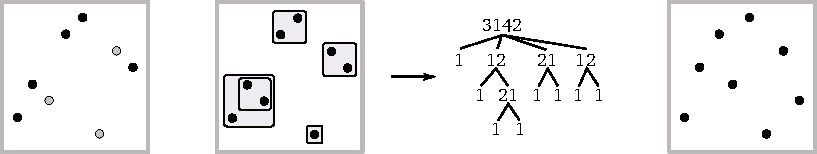
\includegraphics[scale=1.1]{fig_intro.pdf}
\caption{From left to right: (i) plot of permutation $\sigma= (6,1,3,2,8,7,4,5)$ containing $(2,1,3)$ (highlighted) and avoiding $(4,3,2,1)$, (ii) permutation $\sigma$, and (iii) its block decomposition tree; permutation $(3,1,4,2)$ at the root is obtained by contracting the four blocks into points, (iv) simple permutation $(6,1,8,4,2,7,3,5)$.}
\label{fig_intro}
\end{figure}

\subsection{Overview of techniques}
\label{sec:tech}
We sketch the main technical ideas of our proofs.
First, we define roughly the execution log matrix of \greedy. 
The log of executing \greedy on $X \in [n]^m$ is an $n$-by-$m$ matrix $G_X$ such that $G_X(a,t) = 1$ if and only if element $a$ is touched by \greedy at time $t$. The cost of this execution is exactly the number of ones in $G_X$, denoted by $w(G_X)$ (we make this claim precise in \S\,\ref{sec:prelim-short}). 

A submatrix of $G_X$ is obtained by removing some rows and columns of $G_X$.
We say that $G_X$ \emph{contains} a matrix $B$ if there is a submatrix $B'$ of $G_X$ such that $B(i,j) \leq B'(i,j)$ for all $i,j$ (in words, any `one' entry in $B$ must also be a one in $B'$).
 
We say that an algorithm $\aset$ is {\em input-revealing} if there is a constant-size matrix $B$ such that any submatrix of an execution matrix of $\aset$ containing $B$ must contain an access point. 
When such a matrix $B$ exists for an algorithm, we say that $B$ is a {\em capture gadget}.  
The existence for \greedy of a capture gadget $B$ allows us to observe that $G_X$ contains the pattern\footnote{$\otimes$ denotes the tensor (Kronecker) product, to be defined later.} $Q \otimes B$ only if the input sequence contains the pattern defined by $Q$. 
So, if we execute \greedy on an input sequence $X \in \cset_k$ that is $Q$-free for $Q \in S_k$, then $G_X$ cannot contain $Q \otimes B$.  
Now, we can use results from forbidden submatrix theory for bounding $w(G_X)$. 
In short, forbidden submatrix theory is a collection of theorems of the following type: 

\begin{theorem} 
Let $M$ and $P$ be $n$-by-$n$ and $k$-by-$k$ matrices respectively, such that $k \leq n$ (mostly $k$ should be thought of as constant).  
If $M$ does not contain $P$, then $w(M) \leq n f_P(n,k)$.
\end{theorem} 

The function $f_P$ depends on the matrix $P$ that is forbidden in $M$.  
For instance, if $P$ contains at most one $1$-entry per row and column, then $f_P(n,k)$ is only a function of $k$.  
If $P$ contains at most one $1$-entry per column but possibly multiple $1$s per row, then $f_P(n,k) = 2^{\alpha(n)^{O(k)}}$. 
The tightness of the bounds we obtain depends on the structure of the capture gadget $B$. 
This is the reason we have a weaker bound for any $X \in \cset_k$ and stronger bounds when $X$ is more restricted.    
 
We also develop a different set of tools to study the intrinsic complexity of decomposable sequences. Here, in order to compute bounds on \opt, we decompose the execution matrix $M_X$ of an algorithm in a way that mirrors the recursive decomposition of the input sequence $X$. Unfortunately, the behaviour of \greedy is too capricious to afford such a clean decomposition. We therefore modify \greedy to reduce the interference between blocks in the input sequence. The modified algorithm might perform more work locally than \greedy, but globally it is more ``robust''. It is however, an offline algorithm; whether there exists an online algorithm competitive with our robust \greedy, is an interesting open question.


\paragraph{Related work.}
For an overview of results related to dynamic optimality, we refer to the survey of Iacono~\cite{in_pursuit}. 
Besides Tango trees, other $O(\log\log n)$-competitive BST algorithms have been proposed, similarly using Wilber's first bound (multi-splay~\cite{multisplay} and chain-splay~\cite{chain_splay}). Using~\cite{DemaineILO13}, all the known bounds can be simultaneously achieved by combining several BST algorithms. Our study of the execution log of BST algorithms makes use of the geometric view of BST introduced by DHIKP~\cite{DHIKP09}. 

Pattern avoidance in sequences has a large literature in combinatorics~\cite{Vatter,kitaev}, as well as in computer science~\cite{BrunerL13,knuth68, tarjan_sorting, pratt_queues, separable}. The theory of forbidden submatrices can be traced back to a 1951 problem of Zarankiewicz, and its systematic study has been initiated by F\"{u}redi~\cite{furedi}, and Bienstock and Gy\H{o}ri~\cite{bienstock_gyori}. Our use of this theory is inspired by work of Pettie~\cite{pettie_DS, deque_Pet08}, who applied forbidden pattern techniques to prove bounds about data structures (in particular he proves that splay trees achieve $O(n\alpha^{\ast}(n))$ cost on deque-sequences, and he reproves the sequential access theorem for splay trees). There are marked differences in our use of the techniques compared with the work of Pettie. In particular, we look for patterns directly in the execution log of a BST algorithm, without any additional encoding step. Furthermore, instead of using fixed forbidden patterns, we make use of patterns that depend on the input. 

\paragraph{Organization of the paper.} In \S\,\ref{sec:prelim-short} we give a short description of the geometric view of the BST model (following DHIKP~\cite{DHIKP09}), and we introduce concepts used in the subsequent sections. In \S\,\ref{sec:input-rev} we study the input-revealing property of \greedy, and prove our bounds for pattern-avoiding sequences. In \S\,\ref{sec:dec-short} we introduce a robust \greedy, state the decomposition theorem and its applications. Finally, \S\,\ref{sec:conclusions} is reserved for open questions. We defer the proofs of several results, as well as some auxilliary material to the Appendix.


